\documentclass[column,12pt]{article}
\usepackage{indentfirst}
\usepackage[left=.75in,top=.75in,right=1in,bottom=.75in]{geometry}
\usepackage{hyperref}
\usepackage{graphicx}
\hypersetup{
    colorlinks=true,
    linkcolor=blue,
    filecolor=magenta,      
    urlcolor=blue,
}
\graphicspath{ {/} }
\title{CS 591B Final Project\\
\href{http://www.guestmeal.me}{{\it Guestmeal.me }}
}


\author{Ben Lawson \\
		\and 
		Nico Hinderling\\
		\and
		Johnson Lam\\
}
\pdfpagewidth 8.5in
\pdfpageheight 11in 
\oddsidemargin 0in
\evensidemargin 0in

\begin{document}

\maketitle    
%%%%%%%%%%%%%%%%%%%%%%%%%%%%%%%%%%%%%%%%%%%%%%%%%%%%%%%%%%%%%%%%%%%%%%
\section{Abstract}
 
As a freshmen in college, many students are strapped for cash and many struggle to make friends at first. At many colleges, inlcuding Boston University, students living in dormatories are required to obtain a dining plan which, among many benefits, provides ten guest meals per semester. These are not transferable from one semester to another so these will go to waste if unused. These guest meals allow a students to {\it swipe} other students into the dining at no additional cost. {\it Swiping in} is the act of using a guest meal to admit a student to the dining hall.

The dining halls are pristine places to eat. They are all-you-can-eat buffet style and are optimally located around campus. They are very attractive places for people to eat, whether they have a meal plan or not. Students without a meal plan can purchase entry for a variable rate, ranging from \$8.55 to \$15.25. While these prices are reasonable, it can still be a steep cost for some students on a low budget. 

We present a platform that allows students on dining plans to sell their excess guest meals to others who are looking for quick and cheap eats on campus. We describe how to extend this platform to give users the opportunity to make new friends and meet new people over a meal.\\

\section{Motivation}

We believe there is huge potential for social good. Many guest meals go to waste, either to students not caring or not having an opportunity to use them. Each student will be able to optimally utilize their meal plans and students without meal plans can find food at a low cost on campus. Peer-to-peer food service companies currently exist for people to share their home cooked meals with complete strangers. Our goal is to build a similar peer-to-peer business in food services target at the BU community. 

This endeavor gives us a chance to use a few topics discussed in class, in particular auctions, within a real world application. In addition, we have the opportunity to create a product from the ground up and get a taste of what it is like begining a start-up company. Many people take for granted the simplicity of using peer-to-peer platforms, but there are many design and implementation decisions that need to be made by developers to create the platform and keep this
appearance of simplicity. We wanted a technology stack that would accomplish what we needed without too many unnecessary features due to the lack of time to build this app. We also had to decide on how the flow of the auction would work from both the buyer and seller's perspective such that each party will have to put minimal effort into making the transaction. 


%%%%%%%%%%%%%%%%%%%%%%%%%%%%%%%%%%%%%%%%%%%%%%%%%%%%%%%%%%%%%%%%%%%%%%
\section{Market Analysis}

%%%%%%%%%%%%%%%%%%%%%%%%%%%%%%%%%%%%%%%%%%%%%%%%%%%%%%%%%%%%%%%%%%%%%%

Almost a hundred and fifty students have petitioned in the past for a way to convert unused guest meals into dining points (university currency). This inital foundation, along with personal experience, sets the background for our interest in pursuing this opportunity. 

Many applications exist today for people to make quick cash with convenience. Before peer-to-peer networks became proiminent, we saw this in survey and research apps that drew people in with an incentive to either make quick money or have a chance at winning a big prize. But as we know in recent years peer-to-peer applications have exploded and shaken traditional markets in the economy, with Uber and Airbnb being some of the most popular apps. In 2015, Uber had a user base of 8,000,000 people with one million rides daily globally. In that same year, Airbnb had a over 2,000,000 worldwide listings. Such large user bases is what drive these apps to thrive and they are the gold standard for what new peer-to-peer comapnies strive to be. 

Currently there exists a few of peer-to-peer applications that aim towards leveraging dining as a service. VizEat, EatWith, Mealsharing, Feastly, and Traveling Spoon are a few examples of this. The framework for how these peer-to-peer networks operate are similar across all apps in different markets. One market provides a service of some value and another market is interested in consuming such a service. Service providers are screened and verified, their service is listed, and
given a match, a service and monetary payment is exchanged between users. We aim to model our app to the examples listed above, but we are targeting our efforts to connect students on the Boston University campus. Well known problems, such as users not showing up or faulty listings, show up in these peer-to-peer networks no matter the market and will definitely appear in our app as well. We can take these frameworks and solutions that companies have used previously to launch
our app in the quickest manner as possible. An advantage our app with enjoy is the fact that the quality of food will be consistent among all providers, as the food is producted by a third-party (BU Dining Services). \\

\textbf{Questionnaire}

The survey was conducted using the following questions (via Google Forms). We distributed our survey to Boston University student through Facebook. 
\begin{enumerate}
    \item Do you currently have a meal plan?
    \item Approximately how many of your guest meals went to waste at the end of the semester?
    \item Would you be interested in selling your extra guest meals?
    \item If yes, approximately how much would you expect them to sell for? 
    \item Would you pay the price you selected above to purchase a meal?
    \item Why would or wouldn't you pay that price? (optional)
    \item Would you register for an website that traded guest meals for cash?
    \item Why would or wouldn't you? (optional)
\end{enumerate}

\textbf{Survey Results}

A total of 48 Boston University students participated in our survey to identify important aspects related to our application. Of the surveyed participants, about half were on the meal plan and the other half were off the meal plan. Given the split in participants, it gave us a good representation of the interest from both a buyer and seller's perspective. 

\centerline{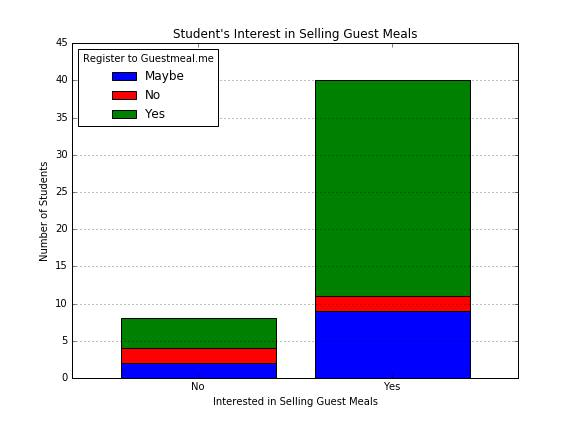
\includegraphics[scale=0.5]{interest.png}}
Over 80\% of the survey participants would be interested in selling their extra guest meals. Along with the fact that over 90\% of respondents said that they would consider registering for our appication, this suggets to us that their is a viable user base and a potential market for this product. 

\centerline{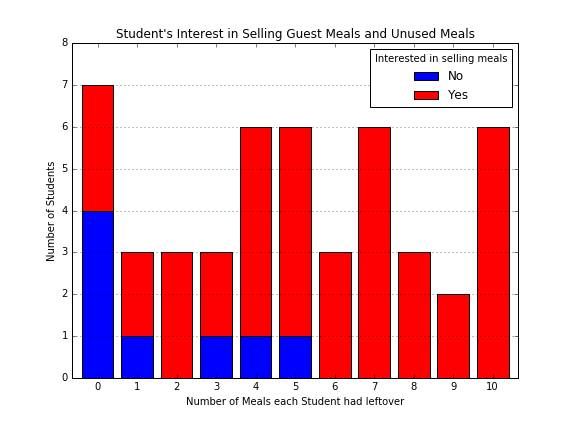
\includegraphics[scale=0.5]{availablemeals.png}}
Of the students not interested in selling their guest meals, a majority of them were those that had very few or none to sell. We can see that students interested in selling their guest meals are the majority in each case, except for students with 0 meals, and over 85\% of students in our survey had more than one guest meal left. This again strongly supports our belief that there would be an interested student population for our application. 

\centerline{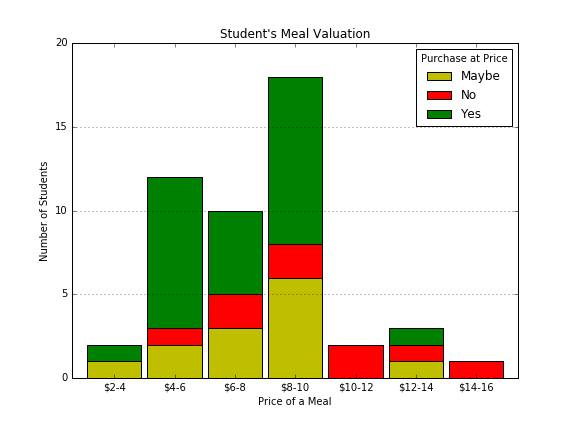
\includegraphics[scale=0.5]{meal_valuation.png}}
We asked repondents what their expected selling price would be and whether they themselves would be willing to pay that price. Over half of the respondents said that they would pay the price they had described, again suggesting that their exists a market. A majority of students suggested that they would sell their guest meals for somewhere in the range of \$4 to \$10- on average a student would sell it for \$6.
If we assume the average number of wasted guest meals in our sample holds true for the population of the first-year class, at \$6 a meal, there would be \$102,485 in potential revenue to be generated from this application for the first-year students alone. At a 2\% commission we would collect \$2,000. 

\section{Goals}
\textbf{Generate Revenue}

First and foremost, we plan to generate revenue in this endeavor. While turning a profit would be nice, we hope to at the least just be able to balance the books. This will be easy initially as there are the tools we have used are free. Once we expand and take on more users, we will have to consider how to efficiently charge for our product and how scalable our technologies will be. \\

\textbf{Connect People}

A huge inspiration for this project is the potential for people to connect over our application. Our reach goal is for strangers to meet and potentially become friends through our product. This will be explored more as a secondary option once a viable product for selling a guest meal is finished and deployed. \\

\textbf{Learning Experience}

Building a project from the ground up is no simple task. From brainstorming ideas to pinpointing exactly what we want to build and implementing them, there were many things to consider. Because our app is being built for business purposes, we had to also consider how viable our product would be from a consumer's perspective and design a flow that would provide the simplest experience for a user, something we don't typically face as computer science students. 


\section{Use Cases}
We briefly outline the different type of meet ups we plan to have from a high level before we set out to develop the app. This may or may not change in our final product \\

\textbf{Dash \& Dine}

The students with guest meals, called {\it providers}, will update their availability whenever they are at the dining hall. Students who plan to purchase meals, called {\it consumers}, will be notified when a meal is available and begin placing bids. We plan to use a dutch auction to faciliate this sale. The dutch auction will be set the current price of a meal at the time of the day. Providers can set a minimium limit When a consumer wins the dutch auction,
they will meet the provider at the dining hall to be swiped in. The provider is not expected to seat and eat their meal with the consumer. \\

\textbf{Personality Matching}

For personality matching, providers and consumers will arrange a time to eat together. This adds more value to the meal, in the form of friendship and comradery. We will use a blind second-price auction in this format, as the meals must be purchased prior and a date will be arranged for the users to meet up in the future. 

% \subsubsection{Mentor Matching}

\section{Technology}
To implement this application, we are developing a web application. We are using a variety of technologies on both the front and back end to faciliatate user authentication, transaction payments, emailing, and auctioning. Our domain can be found at Guestmeal.me and is being hosted on Heroku, a free easy to use cloud-hosting service. \\

\textbf{Web Development}

For the front-end we employ Jinja, SASS, and Bootstrap on a HTML/JS/CSS stack. For the business logic on the back-end we use Python, the flask framework, MongoDB, Send Grid, and Auth0. The current functionality is a basic login framework utilizing Auth0, which can take advantage of social media logins. This will give us the opportunity to use  Facebook and Twitter accounts to facilate personality matchings for later on in development. We chose the flask framework and MongoDB, for
a webserver framework and database storage respectively, due to the low ramp up time it would take to implement along with their ability to meet our technological needs. Send Grid is an easy to use API for sending emails within Python. Bootstrap also takes very little ramp up time to implment and was aesthetically pleasing.\\

\textbf{Databases}

Our web applications consists of two databases. One is managed by Auth0, which handles signups, logins, and emails. Login emails stored here are used to contact users and have users contact each other. A MongoDB NoSQL database, hosted on mlab.com, contains all transactions that have taken place and pricing information for auction purposes. \\

\textbf{Unit Testing}

This currently is a work in progress. Ad-hoc tests have been conducted prior to pushing individual code blocks, but unit tests will be needed to thoroughly test the code, especially once the app is to be deployed. It is especially crucial for unit testing to be conducted on the database features, as small changes to the database model may cause potential errors. \\

\section{First Prototype: Dine \& Dash}
For users to use our app, they must create a login using their email and Auth0 will authenticate them. Later on, we will allow for social media logins to better connect people through their friend groups. 

The first prototype of Guestmeal.me contains three pages: Buy, Sell, and Dashboard. The Buy page displays the price of the current meal available- this decreases throughout the day, following a Dutch auction format, and one meal is sold at a time. A buyer will simply click on a button if they wish to purchase the meal. The Sell page lets a user sell their meal by inputting the lowst price he or she is willing to sell it for and confirming with a click of a button. Once confirmed, the meal will be put out for sale. The Dashboard view will show past transaction by the user.

The price of the meal is set to start at \$10 and slowly decreases throughout the day until it reaches the seller's minimum limit. If not sold by the end of the day 24-hour period since up for sale, it is taken off market and returned to the user. A Dutch auction style is used and the first person to make the transaction will be awarded the meal at that price. After a meal is sold, the next available meal is then put on auction and the process is then repeated. 

When a transaction occur, an automated email will be sent to the buyer and seller containg the contact info of the other party. The two parties will meet up in person and payments will be made in person. 

\section{Marketing and Distribution}
To create interest in our application we will be making an online announcement via various outlets. We will focus on Facebook groups of interest, like "Free Food for All", "Free \& For Sale", as well as the computer science students group. We will also post in "Official Boston University Class of 2020" to target freshmen. Our inital marketing venture will be to target 100 friends (via student groups we belong to) in addition to the online annoucement distributions. Our goal is to get as many user sign ups as possible to get a large enough user base that could facilitate the selling and buying of meals. 

%%%%%%%%%%%%%%%%%%%%%%%%%%%%%%%%%%%%%%%%%%%%%%%%%%%%%%%%%%%%%%%%%%%%%%
\section{Bibliography}
Airbnb, "About Us" airbnb.com. Web. 20 Nov. 2016. \\
 {\it Airbnb is a peer-to-peer online homestay marketplace that allows users to list their homes out for rent. Airbnb was founded in 2008 and is based out of San Francisco, California. They currently have over 60,000,000 guests along with 2,000,000 listings in 191 countries. }\\

Faller, Mike. "Boston University Dining Services: Allow Students to Convert Guest Meals into Dining Points." Online Petition. Change.org. N.p., n.d. Web. 22 Nov. 2016. \\
 {\it Change.org is a well-known website for collecting signatures for a cause or petition. Users have to sign in via social media or create an account. This petition sets the groundwork for our applications and shows the market we are after does exist.}\\

Cardenas, Phillip. "Out Commitment to Safety newsroom.uber.com. Web. 20 Nov. 2016. \\
 {\it Uber is a peer-to-peer online transportation marketplace and is headquartered in San Francisco, California. They were founded in 2009 have have business in over 66 countries. Head of Global Safety, Phillip Cardenas, discusses the safety measures Uber will be reviewing to enhance the safety of both its drivers and riders. 
\end{document}
